\documentclass[twocolumn,a4paper,10pt]{article}
\usepackage[utf8]{inputenc}
\usepackage{amsmath,amssymb}
\usepackage{graphicx}     % Include figure files

\begin{document}
%
Wir werden uns die n\"achsten Semester regelm\"a{\ss}ig in den Vorlesungen Physik 1 bis 3 sehen.  Ich hoffe, da{\ss} Sie alle sich erfolgreich den Stoff erarbeiten werden den Prof.\ Demokritov (Experiment) und ich (Theorie) vorstellen auf unserem Weg durch Mechanik, Thermodynamik, Elektrodynamik, Optik und Spezielle Relativit\"atstheorie.  Im Folgenden m\"ochte ich mich und meine Arbeitsgruppe kurz bei Ihnen vorstellen.

Ich habe um 1990 herum in Dresden Physik studiert, um herauszufinden ``was die Welt im Innersten zusammenh\"alt''. Nachdem ich konsequenterweise mit Elementarteilchenphysik gelieb\"augelt hatte, lie{\ss} ich mich dann f\"ur meine Promotion von der Physik komplexer Systeme anziehen. Arbeitsaufenthalte f\"uhrten mich u.a.\ nach Augsburg, Bayreuth, Berkeley, Dresden und Madrid, bevor ich ab 2007 in Loughborough (UK) lehrte und forschte. Im zeitigen Fr\"uhjahr 2014 verlagerte ich diese Aktivit\"aten nach M\"unster an das Institut f\"ur Theoretische Physik wo wir in der Gruppe \textit{Selbstorganisation und Komplexit\"at} universelle Eigenschaften komplexer Nichtgleichgewichtssysteme mit theoretischen und numerischen Methoden erforschen.  Diese Systemen bestehen oft aus vielen mikroskopischen, nichtlinear wechselwirkenden Komponenten was ausserhalb (und fern) vom Gleichgewicht zur spontanen Entwicklung von Strukturen f\"uhrt, die nicht von au{\ss}en aufgepr\"agt werden, sondern durch Selbstorganisationsprozesse entstehen.  Im allt\"aglichen Leben kommen solche Ph\"anomene in vielfacher Weise vor, z.B. als Konvektion im Milchkaffee, bei der Ausbildung (und Dynamik) von Tierfellmustern, Wasserwellen, Sandd\"unen oder Wolkenb\"andern.

\begin{figure}[tbh]
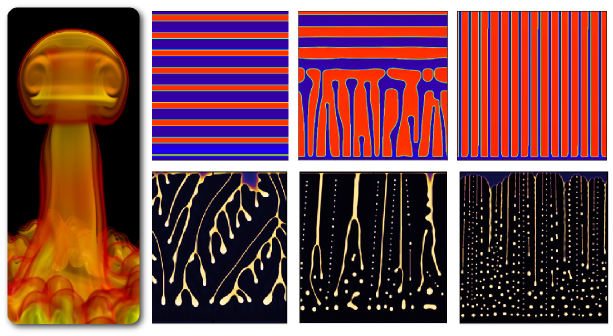
\includegraphics[width=\hsize]{g3184}
\caption{Beispiele berechneter Strukturen: Pilzstruktur bei thermischer Konvektion (links), Fingerinstabilit\"at beim Entnetzen und Verdunsten einer Nanoteilchensuspension (unten rechts) und Streifenmuster beim Transfer oberfl\"achenaktiver Substanzen von einem Bad auf eine bewegte Platte (unten rechts). Bilder von J. L\"ulff, A. Archer, M. Wilczek.
}
\label{fig:examples}
\end{figure}

Ein Schwerpunkt der Gruppe ist weiche und aktive Materie deren Dynamik oft grenzfl\"achendominiert ist, d.h.\ sie wird durch Grenzfl\"achenenergien kontrolliert. Beispiele sind Tropfen auf Substraten, Schichten von Fl\"ussig\-kristallen und kolloidalen Suspensionen. Ein wichtiges Ziel ist das Verst\"andnis der strukturbildenden Wechselwirkungen diverser voneinander abh\"angiger  Transportprozesse und Phasen\"uberg\"ange. \"Ahnliche Fragen treten auch bei der Dynamik biologischer Zellen, dem Gewebe\-wachstum sowie bei der Bewegung von Schw\"armen auf. Von gro{\ss}em Interesse ist auch die Strukturbildung durch Selbstassemblierung mikroskopischer Bestandteile. Deren Kontrolle wird benutzt,  um gro{\ss}fl\"achig Oberfl\"achen mit wohlstrukturierten Schichten zu bedecken. Wir m\"ochten verstehen wie die grundlegenden Eigenschaften der Materialien und Prozesse zur Bildung spezieller funktionaler Muster f\"uhren und man diese durch aufgepr\"agte Felder kontrollieren kann.

Au\ss{}erdem besch\"aftigen wir uns mit thermi\-scher Konvektion (durch Temperaturgradienten angetriebene Str\"omungen) und Turbulenz. Fast alle solche Fl\"usse in der Natur (z.B. Atmosph\"are, Ozeane, Plattentektonik) sind turbulent und aufgrund ihres chaotischen Verhaltens schwer zu behandeln. Insbesondere sind genaue Vorhersagen \"uber l\"angere Zeiten fast unm\"oglich (siehe Wetterbericht..). Stattdessen ist unser Ziel, neue kombinierte statistische und numerische Beschreibungen zu entwickeln die dann auf Supercomputern numerisch gel\"ost werden und zu einem besseren Verst\"andnis turbulenter Systeme f\"uhren. 

Obwohl in der Beschreibung nicht leicht erkennbar, m\"ochte ich Ihnen abschlie{\ss}end versichern, dass der
Weg zum Verst\"andnis solch komplexer Ph\"anomene in den Grundvorlesungen beginnt die wir demn\"achst gemeinsam
bestreiten. Daf\"ur w\"unsche ich Ihnen viel Erfolg. Sollten Sie mehr \"uber komplexe Systeme erfahren wollen sind Sie herzlich eingeladen, die Arbeitsgruppe zu besuchen.

\end{document}
